%%%%%%%%%%%%%%%%%%%%%%%% index.tex %%%%%%%%%%%%%%%%%%%%%%%%%%%%%
%
% root file for OOPSLA contributed book.
%
%%%%%%%%%%%%%%%%%%%%%%%%%%%%%%%%%%%%%%%%%%%%%%%%%%%%%%%%%%%%%%%%

%%%%%%%%%%%%%%%%%%%%%%%%%%%%%%%%%%%%%%%%%%%%%%%%%%%%%%%%%%%%%%%%
%% you can use compile.sh (> sh compile.sh) to compile it to .dvi, .ps, .pdf.
%% requires Perl installed on machine + latexmk package installed with Latex Package Manager.
%%%%%%%%%%%%%%%%%%%%%%%%%%%%%%%%%%%%%%%%%%%%%%%%%%%%%%%%%%%%%%%%

%% See refguide for list of available options.
\documentclass[
graybox,
envcountchap,
%natbib
]{svmult}

%\usepackage{type1cm}        % activate if the above 3 fonts are 
                             % not available on your system

\usepackage{makeidx}         % allows index generation
\usepackage{graphicx}        % standard LaTeX graphics tool
                             % when including figure files
\usepackage{multicol}        % used for the two-column index
\usepackage[bottom]{footmisc}% places footnotes at page bottom

\usepackage{newtxtext}       % 
\usepackage{newtxmath}       % selects Times Roman as basic font

\usepackage{footmisc}
% \usepackage{natbib}

%% Additional packages added. Add necessary packages here.
%\usepackage[english]{babel}
\usepackage{xcolor}
\usepackage{tabularx}
\usepackage{listings}
\usepackage{booktabs}
\usepackage{bibunits}
\usepackage{hyperref}
\usepackage{url}
\usepackage{mathtools}
\usepackage{import}
\usepackage{lipsum}

%% define commands here.
\newcommand*{\CHAPTERSROOT}{chapters}	% root path for chapters.

%% consistent book-wide bibliography style.
\bibliographystyle{./styles/spmpsci} % single consistent bibtex bibliography style

\makeindex             % used for the subject index

%%%%%%%%%%%%%%%%%%%%%%%%%%%%%%%%%%%%%%%%%%%%%%%%%%%%%%%%%%%%%%%%%%
\begin{document}
\frontmatter%%%%%%%%%%%%%%

%%%%%%
\begin{titlepage}
	\author{Authors Here}
	\title{PL4DS Shannon Book}
	\date{September 2019}
	
	%% publisher is defined in the class file
\end{titlepage}
%%%%%%
%%%%%%%%%%%%%%%%%%%%%%% dedication.tex %%%%%%%%%%%%%%%%%%%%%%%%%%
%
% dedication
%
%%%%%%%%%%%%%%%%%%%%%%%%%%%%%%%%%%%%%%%%%%%%%%%%%%%%%%%%%%%%%%%%%

\begin{dedication}
Book dedication goes here.
\end{dedication}




%%%%%%%%%%%%%%%%%%%%%%% foreword.tex %%%%%%%%%%%%%%%%%%%%%%%%%%
%
% foreword
%
%%%%%%%%%%%%%%%%%%%%%%%%%%%%%%%%%%%%%%%%%%%%%%%%%%%%%%%%%%%%%%%

\foreword

foreword, if applicable, goes here.

\vspace{\baselineskip}
\begin{flushright}\noindent
Place, month year\hfill {\it Firstname  Surname}\\
\end{flushright}



%%%%%%%%%%%%%%%%%%%%%%% preface.tex %%%%%%%%%%%%%%%%%%%%%%%%%%
%
% preface
%
%%%%%%%%%%%%%%%%%%%%%%%%%%%%%%%%%%%%%%%%%%%%%%%%%%%%%%%%%%%%%%

\preface

preface (preliminary statement about origin, scope, purpose, plan, and intended audience), if applicable, goes here.

\vspace{\baselineskip}
\begin{flushright}\noindent
Place(s),\hfill {\it Firstname  Surname}\\
month year\hfill {\it Firstname  Surname}\\
\end{flushright}



%%%%%%%%%%%%%%%%%%%%%%% acknowledgement.tex %%%%%%%%%%%%%%%%%%%%%%%%%%
%
% acknowledgements
%
%%%%%%%%%%%%%%%%%%%%%%%%%%%%%%%%%%%%%%%%%%%%%%%%%%%%%%%%%%%%%%%%%%%%%%

\extrachap{Acknowledgements}

Acknowledgements, if applicable, go here.



%%%%%%%%%%%%%%%%%%%%%%% contriblist.tex %%%%%%%%%%%%%%%%%%%%%%%%%%
%
% contributor's list.
%
%%%%%%%%%%%%%%%%%%%%%%%%%%%%%%%%%%%%%%%%%%%%%%%%%%%%%%%%%%%%%%%%%%
\contributors

\begin{thecontriblist}
Firstname Surname
\at ABC Institute, 123 Prime Street, Daisy Town, NA 01234, USA, \email{smith@smith.edu}
\and
Firstname Surname
\at XYZ Institute, Technical University, Albert-Schweitzer-Str. 34, 1000 Berlin, Germany, \email{meier@tu.edu}
\end{thecontriblist}
%%%%%%%%%%%%%%%%%%%%%%acronym.tex%%%%%%%%%%%%%%%%%%%%%%%%%%%%%%%%%%%%%%%%%
% sample list of acronyms
%
% Use this file as a template for your own input.
%
%%%%%%%%%%%%%%%%%%%%%%%% Springer Nature%%%%%%%%%%%%%%%%%%%%%%%%%%

\extrachap{Acronyms}

A list of Acronyms, if needed, goes here.

\begin{description}[CABR]
\item[ABC]{Spelled-out abbreviation and definition}
\item[BABI]{Spelled-out abbreviation and definition}
\item[CABR]{Spelled-out abbreviation and definition}
\end{description}

\tableofcontents

\mainmatter%%%%%%%%%%%%%%%
%%%%%%%%%%%%%%%%%%%%%%% part1.tex %%%%%%%%%%%%%%%%%%%%%%%%%%
%
% Part 1
%
%%%%%%%%%%%%%%%%%%%%%%%%%%%%%%%%%%%%%%%%%%%%%%%%%%%%%%%%%%%%

\begin{partbacktext}
\part{Part Title}
\noindent This is an optional part title page that can contain a Part description of max. 1 page.

\end{partbacktext}

%%%% List of contributions %%%%%
%%%% Use subimport to include chapter indexes, so that paths within that are relative to the chapter dir.
\import{chapters/chapter01/}{index}
%%%%%%%%%%%%%%%%%%%%%%%%%%%%%%%%

\backmatter%%%%%%%%%%%%%%%
\appendix
%%%%%%%%%%%%%%%%%%%%% appendix.tex %%%%%%%%%%%%%%%%%%%%%%%%%%%%%%%%
%
% global appendix.
%
%%%%%%%%%%%%%%%%%%%%%%%%%%%%%%%%%%%%%%%%%%%%%%%%%%%%%%%%%%%%%%%%%%%

\chapter{Chapter Heading}
\label{global:appendix} % Always give a unique label, prefixed with global.

The global appendix of the book goes here.

\section{Section Heading}\label{global:appendix:A1}

Instead of simply listing headings of different levels we recommend to let every heading be followed by at least a short passage of text. Further on please use the \LaTeX\ automatism (cite, ref, etc.) for all your cross-references and citations.

\subsection{Subsection Heading}\label{global:appendix:A2}
Instead of simply listing headings of different levels we recommend to let every heading be followed by at least a short passage of text. Further on please use the \LaTeX\ automatism for all your cross-references and citations as has already been described in Sect.~\ref{global:appendix:A1}.

For multiline equations we recommend to use the \verb|eqnarray| environment.
\begin{eqnarray}
\vec{a}\times\vec{b}=\vec{c} \nonumber\\
\vec{a}\times\vec{b}=\vec{c}
\label{global:appendix:eq:1}
\end{eqnarray}

\subsubsection{Subsubsection Heading}\label{global:appendix:A2:1}

% For figures use
%
\begin{figure}[t]
\sidecaption[t]
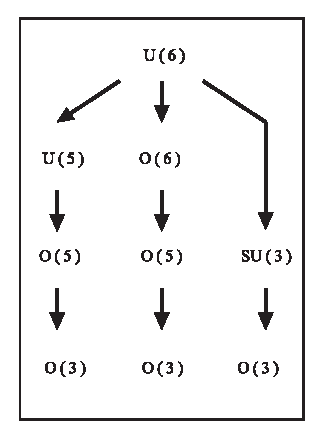
\includegraphics[scale=.65]{editorial/assets/figure}
%
% If no graphics program available, insert a blank space i.e. use
%\picplace{5cm}{2cm} % Give the correct figure height and width in cm
%
\caption{Please write your figure caption here}
\label{global:appendix:fig:1}
\end{figure}

% For tables use
%
\begin{table}
\caption{Please write your table caption here}
\label{global:appendix:table:1}       % Give a unique label
%
% Follow this input for your own table layout
%
\begin{tabular}{p{2cm}p{2.4cm}p{2cm}p{4.9cm}}
\hline\noalign{\smallskip}
Classes & Subclass & Length & Action Mechanism  \\
\noalign{\smallskip}\hline\noalign{\smallskip}
Translation & mRNA$^a$  & 22 (19--25) & Translation repression, mRNA cleavage\\
Translation & mRNA cleavage & 21 & mRNA cleavage\\
Translation & mRNA  & 21--22 & mRNA cleavage\\
Translation & mRNA  & 24--26 & Histone and DNA Modification\\
\noalign{\smallskip}\hline\noalign{\smallskip}
\end{tabular}
$^a$ Table foot note (with superscript)
\end{table}
%

%%%%%%%%%%%%%%%%%%%%%%acronym.tex%%%%%%%%%%%%%%%%%%%%%%%%%%%%%%%%%%%%%%%%%
%
% global glossary.
%
%%%%%%%%%%%%%%%%%%%%%%%%%%%%%%%%%%%%%%%%%%%%%%%%%%%%%%%%%%%%%%%%%%%%%%%%%%%%

\Extrachap{Glossary}

Use this for a global glossary, if applicable.

\runinhead{glossary term} Write here the description of the glossary term. Write here the description of the glossary term. Write here the description of the glossary term.

\runinhead{glossary term} Write here the description of the glossary term. Write here the description of the glossary term. Write here the description of the glossary term.

\runinhead{glossary term} Write here the description of the glossary term. Write here the description of the glossary term. Write here the description of the glossary term.

\runinhead{glossary term} Write here the description of the glossary term. Write here the description of the glossary term. Write here the description of the glossary term.

\runinhead{glossary term} Write here the description of the glossary term. Write here the description of the glossary term. Write here the description of the glossary term.
\printindex

\end{document}
%%%%%%%%%%%%%%%%%%%%%%%%%%%%%%%%%%%%%%%%%%%%%%%%%%%%%%%%%%%%%%%%%%
